% interactcadsample.tex
% v1.03 - April 2017

\documentclass[]{interact}

\usepackage{epstopdf}% To incorporate .eps illustrations using PDFLaTeX, etc.
\usepackage{subfigure}% Support for small, `sub' figures and tables
%\usepackage[nolists,tablesfirst]{endfloat}% To `separate' figures and tables from text if required

\usepackage{natbib}% Citation support using natbib.sty
\bibpunct[, ]{(}{)}{;}{a}{}{,}% Citation support using natbib.sty
\renewcommand\bibfont{\fontsize{10}{12}\selectfont}% Bibliography support using natbib.sty

\theoremstyle{plain}% Theorem-like structures provided by amsthm.sty
\newtheorem{theorem}{Theorem}[section]
\newtheorem{lemma}[theorem]{Lemma}
\newtheorem{corollary}[theorem]{Corollary}
\newtheorem{proposition}[theorem]{Proposition}

\theoremstyle{definition}
\newtheorem{definition}[theorem]{Definition}
\newtheorem{example}[theorem]{Example}

\theoremstyle{remark}
\newtheorem{remark}{Remark}
\newtheorem{notation}{Notation}

% see https://stackoverflow.com/a/47122900

% Pandoc citation processing

\usepackage{hyperref}
\usepackage[utf8]{inputenc}
\def\tightlist{}
\newcommand*{\Perm}[2]{{}^{#1}\!P_{#2}}%


\begin{document}

\articletype{ARTICLE TEMPLATE}

\title{Effectiveness of visual test in linear regression diagnositics}


\author{\name{Weihao Li$^{a}$, Dianne Cook$^{a}$, Emi Tanaka$^{a}$}
\affil{$^{a}$Department of Econometrics and Business Statistics, Monash
University, Clayton, VIC, Australia}
}

\thanks{CONTACT Weihao
Li. Email: \href{mailto:weihao.li@monash.edu}{\nolinkurl{weihao.li@monash.edu}}, Dianne
Cook. Email: \href{mailto:dicook@monash.edu}{\nolinkurl{dicook@monash.edu}}, Emi
Tanaka. Email: \href{mailto:emi.tanaka@monash.edu}{\nolinkurl{emi.tanaka@monash.edu}}}

\maketitle

\begin{abstract}
Abstract to fill.
\end{abstract}

\begin{keywords}
visual inference; regression diagnostics;
\end{keywords}

\hypertarget{introduction}{%
\section{Introduction}\label{introduction}}

Regression diagnostics is an essential step in regression analysis which
is a field of study with at least a hundred years of history. The
diagnostic procedure conventionally involves evaluating the fitness of
the proposed model, detecting the presence of influential observations
and outliers, checking the validity of model assumptions and many more.
In terms of diagnostic techniques, data plots, hypothesis testing, and
summary statistics are vital tools for a systematic and detailed
examination of the regression model \citep{mansfield1987diagnostic}.

Many of those regression diagnostic methods and procedures are mature
and well-established in books first published in the twentieth century,
such as \citet{draper1998applied}, \citet{montgomery1982introduction},
\citet{belsley_regression_1980}, \citet{cook_applied_1999} and
\citet{cook1982residuals}. Regardless of the level of difficulty, one
will find the importance and usefulness of diagnostic plots being
emphasized in those books repeatedly. Checking diagnostic plots is also
the recommended starting point for validating model assumptions such as
normality, homoscedasticity and linearity
\citep{anscombe_examination_1963}.

\hypertarget{diagnostic-plots}{%
\subsection{Diagnostic plots}\label{diagnostic-plots}}

Graphical summaries in which residuals are plotted against fitted values
or other functions of the predictor variables that are approximately
orthogonal to residuals are referred to as standard residual plots in
\citet{cook1982residuals}. As suggested by \citet{cook1982residuals},
these kinds of diagnostic plots are commonly used to identify patterns
that are indicative of nonconstant error variance or non-linearity. Raw
residuals and studentized residuals are the two most frequently used
residuals in standard residual plots. The debt on which type of
residuals should be used is always present. While raw residuals are the
most common computer regression software package output, by applying a
scaling factor, the ability to reveal nonconstant error variance in
standard residual plots will often be enhanced by studentized residuals
in small sample size \citep{gunst1980regression}. As a two-dimensional
representation of a model in a \(p\)-dimensional space, standard
residual plots project data points onto the variable of the horizontal
axis, which is a vector in \(p\)-dimensional space. Observations with
the same projection will be treated as equivalent as they have the same
abscissa. Consequently, standard residual plots are often useful in
revealing model inadequacies in the direction of the variable of the
horizontal axis but could be inadequate for detecting patterns in other
directions, especially in those perpendicular to the variable of the
horizontal axis. Hence, in practice, multiple standard residual plots
with different horizontal axes will be examined
\citep{cook1982residuals}. Overlapping data points is another general
issue in scatter plots not limited to standard residual plots, which
often makes plots difficult to interpret because visual patterns are
concealed. Thus, for a relatively large sample size,
\citet{cleveland1975graphical} suggests the use of robust moving
statistics as reference lines to give aid to the eye in seeing patterns,
which nowadays, are usually replaced with a spline or local polynomial
regression line.

Other types of data plots that are often used in regression diagnostics
include partial residual plots and probability plots. Partial residual
plots are useful supplements to standard residual plots as they provide
additional information on the extent of the non-linearity. Probability
plots can be used to compare the sampling distribution of the residuals
to the normal distribution for assessing the normality assumptions.

\hypertarget{hypothesis-testing}{%
\subsection{Hypothesis testing}\label{hypothesis-testing}}

Other than checking diagnostic plots, analysts may perform formal
hypothesis testing for detecting model defects. Depending on the
alternative hypothesis that is focused on, a variety of tests can be
applied. For example, the presence of heteroskedasticity can usually be
tested by applying the White test
\citep{white_heteroskedasticity-consistent_1980} or the Breusch-Pagan
test \citep{breusch_simple_1979}, which are both derived from the
Lagrange multiplier test \citep{silvey1959lagrangian} principle that
relies on the asymptotic properties of the null distribution. For
testing non-linearity, one may apply the F-test to examine the
significance of specific polynomial and non-linear forms of the
regressors, or the significance of proxy variables as in the Ramsey
Regression Equation Specification Error Test (RESET)
\citep{ramsey_tests_1969}.

As discussed in \citet{cook1982residuals}, most residual-based tests for
a particular type of departure from model assumptions are sensitive to
other types of departures. It is likely the null hypothesis is correctly
rejected but for the wrong reason, which is known as the ``Type III
error''. Additionally, outliers will often incorrectly trigger the
rejection of the null hypothesis despite the residuals are well-behaved
\citep{cook_applied_1999}. This can be largely avoided in diagnostic
plots as experienced analysts can evaluate the acceptability of
assumptions flexibly, even in the presence of outliers.
\citet{montgomery1982introduction} suggested that based on their
experience, statistical tests are not widely used in regression
diagnostics. The same or even larger amount of information can be
provided by diagnostic plots than the corresponding tests in most
empirical studies. Not to mention, it is almost impossible to have an
exactly correctly specified model in reality. There is a well-known
aphorism in statistics stated by George Box - ``All models are wrong,
but some are useful''. This indicates proper hypothesis tests will
always reject the null hypothesis as long as the sample size is large
enough. The outcome ``Not reject'' can be interpreted as either ``effect
size is small'' or ``sample size is small''. and the outcome ``reject''
doesn't inform us whether and how much the model defects are of actual
consequence to the inference and prediction. But still, the
effectiveness of statistical tests shall not be disrespected.
Statistical tests have a chance to provide analysts with unique
information. In situations where no suitable diagnostic plots can be
found for a particular violation of the assumptions, or excessive
diagnostic plots are needed to be checked, one will have no choice but
to fall back on statistical tests if there exists any. A good regression
diagnostic practice should be a balanced combination of both methods.

\hypertarget{visual-inference}{%
\subsection{Visual inference}\label{visual-inference}}

However, unlike hypothesis testing built upon rigorous statistical
procedures, reading diagnostic plots relies on graphical perception -
human's ability to interpret and decode the information embedded in the
graph \citep{cleveland_graphical_1984}, which is to some extent
subjective and indecisive. Further, visual discovery suffers from its
unsecured and unconfirmed nature where the degree of the presence of the
visual features typically can not be measured quantitatively and
objectively, which may lead to over or under-interpretations of the
data. One such example is finding an over-interpretation of the
separation between gene groups in a two-dimensional projection from a
linear discriminant analysis when in fact there are no differences in
the expression levels between the gene groups and separation is not an
uncommon occurrence \citep{roy_chowdhury_using_2015}.

Visual inference was first introduced in a 1999 Joint Statistical
Meetings (JSM) talk with the title ``Inference for Data Visualization''
by \citet{buja_inference_1999} as an idea to address the issue of valid
inference for visual discoveries of data plots
\citep{gelman_exploratory_2004}. Later, in the Bayesian context, data
plots was systematically considered as model diagnostics by taking
advantage of the data simulated from the assumed statistical models
\citep{gelman_bayesian_2003, gelman_exploratory_2004}.

It was surprising that the essential components of visual inference had
actually been established in \citet{buja_inference_1999}, but it was not
until 10 years later that \citet{buja_statistical_2009} formalized it as
an inferential framework to extend confirmatory statistics to visual
discoveries. This framework redefines the test statistics, tests, null
distribution, significance levels and \(p\)-value for visual discovery
modelled on the confirmatory statistical testing. Figure
\ref{fig:parallelism} outlines the parallelism between conventional
tests and visual discovery.

\begin{figure}
\centering
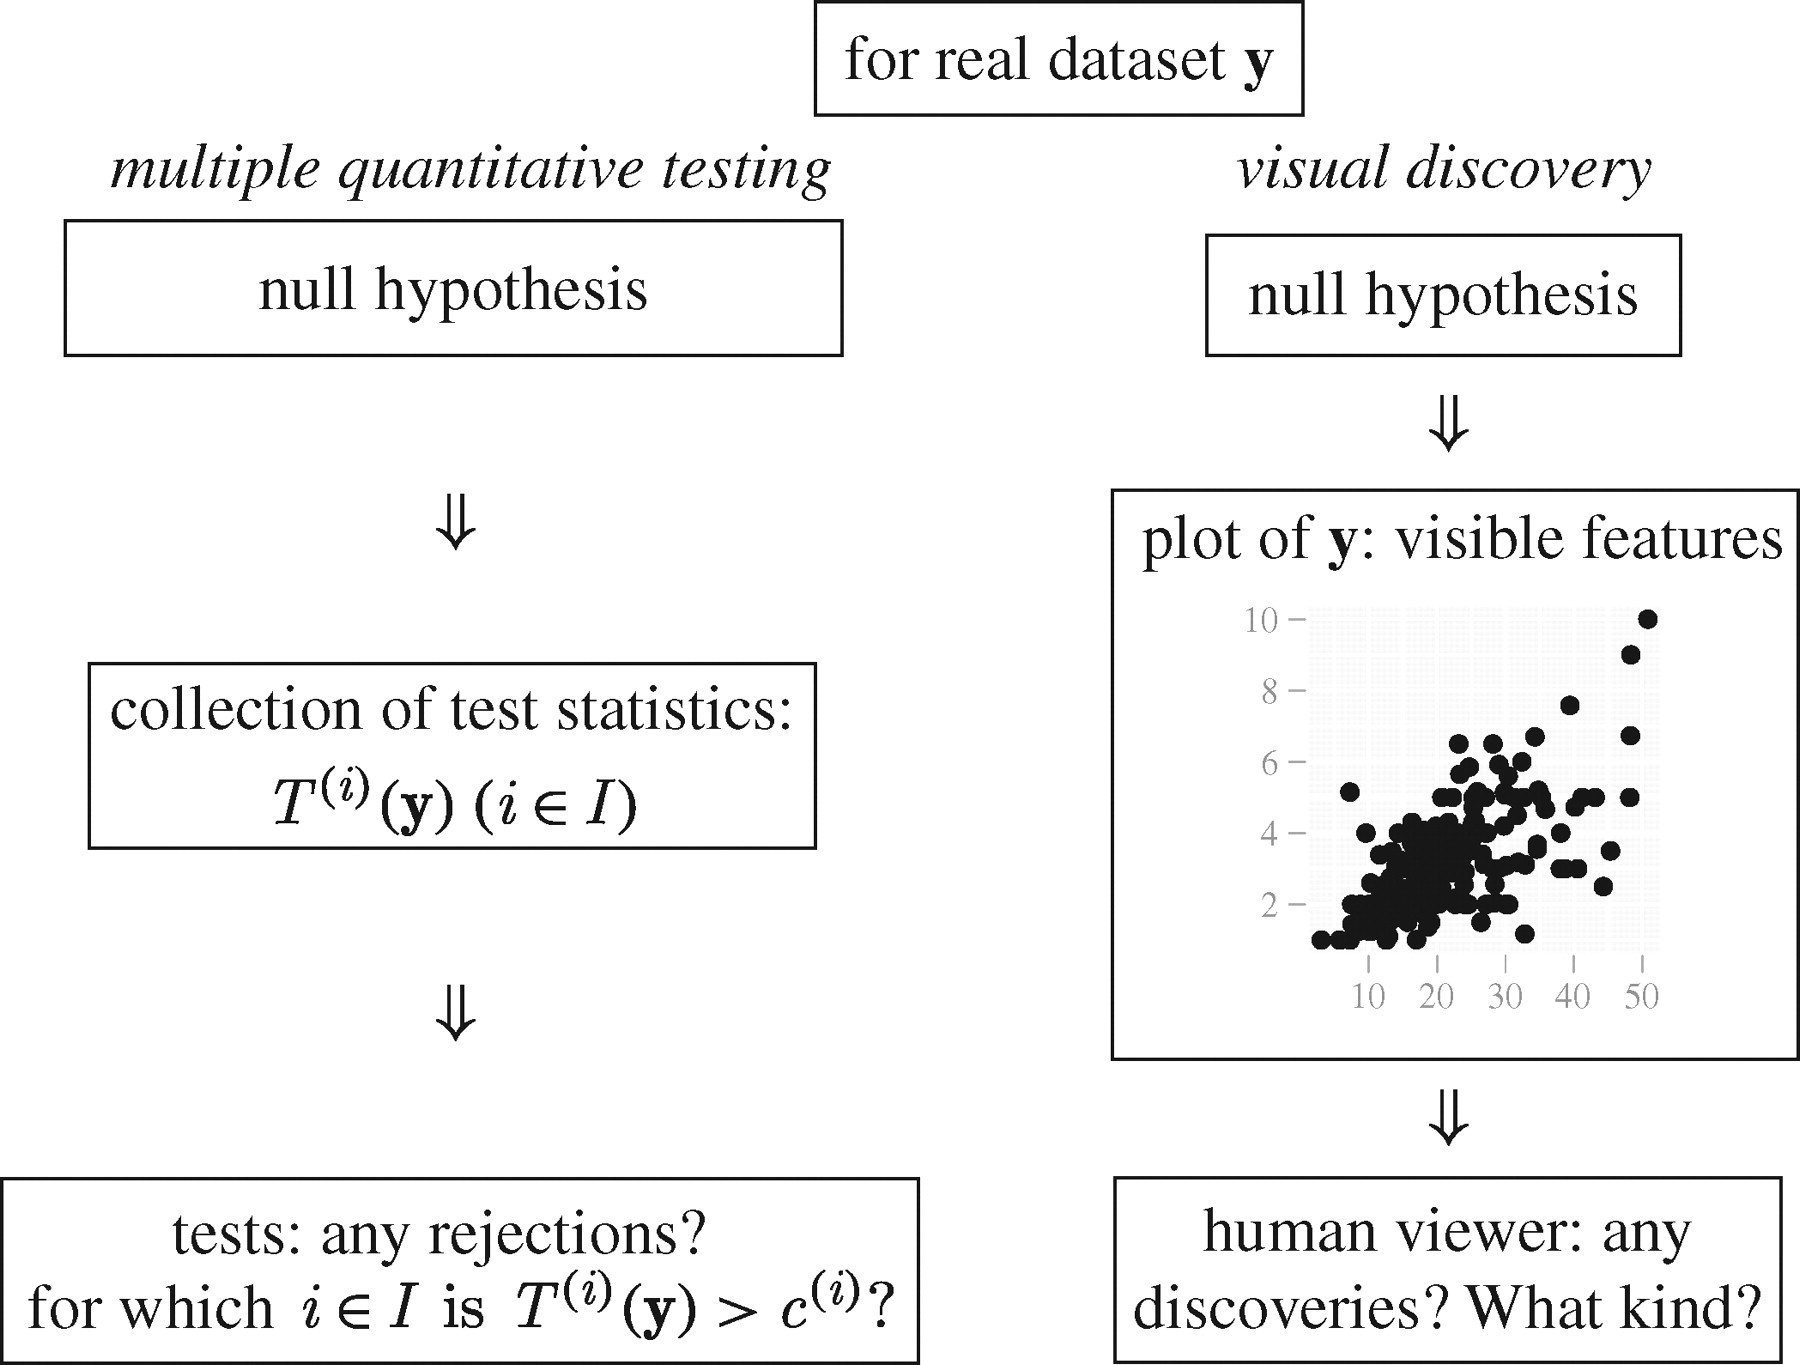
\includegraphics[width=4.6875in,height=3.55208in]{figures/rsta2009012001.jpg}
\caption{Parallelism between multiple quantitative testing and visual
discovery \citep{buja_statistical_2009}. Visible features in a plot are
viewed as a collection of test statistics
\(T^{(i)}(\boldsymbol{\mathrm{y}})~(i \in I)\), and any visual
discoveries that are inconsistent with the null hypothesis are treated
as evidence against the null. For regression diagnostics, the null
hypothesis would be the assumed model, and visual discoveries could be
any visual features in favour of any alternatives.
\label{fig:parallelism}}
\end{figure}

In visual inference, a collection of test statistics
\(T^{(i)}(\boldsymbol{\mathrm{y}})~(i \in I)\) is defined, where
\(\boldsymbol{\mathrm{y}}\) is the data and \(I\) is a set of all
possible visual features. \citet{buja_statistical_2009} described each
of the test statistics \(T^{(i)}(\boldsymbol{\mathrm{y}})\) as a
measurement of the degree of presence of a visual feature.
Alternatively, \citet{majumder_validation_2013} avoids the use of visual
features and defined the visual statistics \(T(.)\) as a mapping from a
dataset to a data plot. Both definitions of visual test statistics are
valid, but in the rest of the paper the first definition will be used as
it covers some details needed by the following discussion. A visual
discovery is defined as a rejection of a null hypothesis, and the same
null hypothesis can be rejected by many different visual discoveries
\citep{buja_statistical_2009}. For regression diagnostics, the null
hypothesis would be the assumed model, while the visual discoveries
would be any findings that are inconsistent with the null hypothesis.
The same regression model can be rejected by many reasons with residual
plot, including non-linearity and heteroskedasticity as shown in Figure
\ref{fig:residual-plot-cubic-heter}.

\begin{figure}
\centering
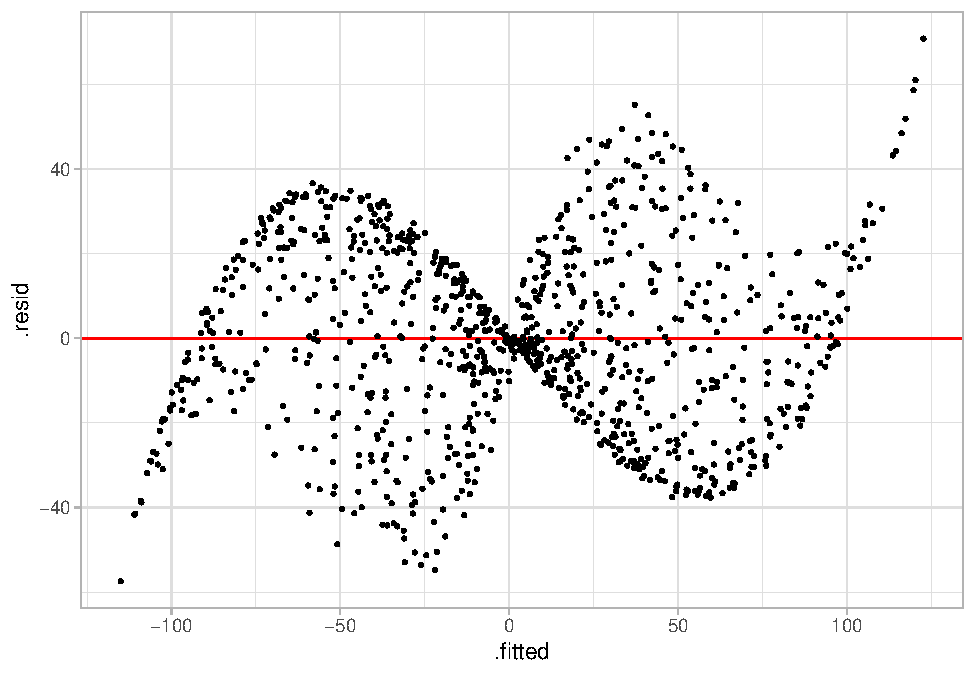
\includegraphics{paper_comparison_files/figure-latex/residual-plot-cubic-heter-1.pdf}
\caption{Residuals vs.~fitted values plot for a classical linear
regression model. The residuals are produced by fitting a two-predictor
multiple linear regression model with data generated from a cubic linear
model. From the residual plot, ``butterfly shape'' can be observed which
generally would be interpretd as evidence of heteroskedasticity.
Further, from the outline of the shape, nonlinear patterns exist. Both
visual discoveries are evidence against the null hypothesis, though
heteroskedasticity actually does not exist in the data generating
process. \label{fig:residual-plot-cubic-heter}}
\end{figure}

\hypertarget{se:sampling-from-null}{%
\subsubsection{Sampling from the null
distribution}\label{se:sampling-from-null}}

The null distribution of plots refers to the infinite collection of
plots of null datasets sampled from \(H_0\). It is defined as the
analogue of the null distribution of test statistics in conventional
test \citep{buja_statistical_2009}. In practice, a finite number of
plots of null datasets could be generated, called null plots. In the
context of regression diagnostics, sampling data from \(H_0\) is
equivalent to sampling data from the assumed model. As
\citet{buja_statistical_2009} suggested, \(H_0\) is usually composited
by a collection of distributions controlled by nuisance parameters.
Since regression models can have various forms, there is no general
solution to this problem, but it sometimes can be reduced to so called
``reference distribution'' by applying one of the three methods: (i)
sampling from a conditional distribution given a minimal sufficient
statistic under \(H_0\), (ii) parametric bootstrap sampling with
nuisance parameters estimated under \(H_0\), and (iii) Bayesian
posterior predictive sampling.

The conditional distribution given a minimal sufficient statistic is the
best justified reference distribution among the three
\citep{buja_statistical_2009}. Suppose there exists a minimal sufficient
statistic \(\boldsymbol{S}(\boldsymbol{y})\) under the null hypothesis,
any null datasets \(\boldsymbol{y^{*}}\) should fulfil the condition
\(\boldsymbol{S}(\boldsymbol{y}) = \boldsymbol{s}\). Using the classical
normal linear regression model as example, the minimal sufficient
statistic is
\(\boldsymbol{S}(\boldsymbol{y}) = (\hat{\boldsymbol{\beta}}, \boldsymbol{e}'\boldsymbol{e})\),
where \(\hat{\boldsymbol{\beta}}\) are the coefficient estimators and
\(\boldsymbol{e}'\boldsymbol{e}\) is the residual sum of square.
Alternatively, the minimal sufficient statistic can be constructed as
\(\boldsymbol{S}(\boldsymbol{y}) = (\hat{\boldsymbol{y}}, ||\boldsymbol{e}||)\),
where \(\hat{\boldsymbol{y}}\) are the fitted values and
\(||\boldsymbol{e}||\) is the length of residuals, which is more
intuitive as suggested by \citet{buja_statistical_2009}. Since the
fitted values are held fixed, the variation can only occur in the
residual space. And because the length of residual is also held fixed,
residuals obtained from a null dataset has to be a random rotation of
\(\boldsymbol{e}\) in the residual space. With this property, null
residuals can be simulated by regressing \(N\) i.i.d standard normal
random draws on the regressors, then rescaling it by the ratio of
residual sum of square in two regressions.

\hypertarget{se:lineup}{%
\subsubsection{Lineup protocol}\label{se:lineup}}

With the simulation mechanism of null plots being provided, another
aspect of hypothesis testing that needs to be addressed is the control
of false positive rate or Type I error. Any visual statistic
\(T^{(i)}(\boldsymbol{\mathrm{y}})\) needs to pair with a critical value
\(c^{(i)}\) to form a hypothesis test. When a visual feature \(i\) is
discovered by the observer from a plot, the corresponding visual
statistic \(T^{(i)}(\boldsymbol{\mathrm{y}})\) may not be known as there
is no general agreement on the measurement of the degree of presence of
a visual feature. It is only the event that
\(T^{(i)}(\boldsymbol{\mathrm{y}}) > c^{(i)}\) is confirmed. Similarly,
if any visual discovery is found by the observer, we say, there exists
\(i \in I:~T^{(i)}(\boldsymbol{\mathrm{y}}) > c^{(i)}\)
\citep{buja_statistical_2009}.

Using the above definition, the family-wise Type I error can be
controlled if one can provide the collection of critical values
\(c^{(i)}~(i \in I)\) such that
\(P(\mathrm{there~exists~} i \in I: T^{(i)}(\boldsymbol{\mathrm{y}}) > c^{(i)}|\boldsymbol{\mathrm{y}}) \leq \alpha\),
where \(\alpha\) is the significance level. However, since the quantity
of \(T^{(i)}(\boldsymbol{\mathrm{y}})\) may not be known, such
collection of critical values can not be provided.

\citet{buja_statistical_2009} proposed the lineup protocol as a visual
test to calibrate the Type I error issue without the specification of
\(c^{(i)}~(i \in I)\). It is inspired by the ``police lineup'' or
``identity parade'' which is the act of asking the eyewitness to
identify criminal suspect from a group of irrelevant people. The
protocol consists of \(m\) randomly placed plots, where one plot is the
actual data plot, and the remaining \(m - 1\) plots have the identical
graphical production as the data plot except the data has been replaced
with data consistent with the null hypothesis. Then, an observer who
have not seen the actual data plot will be asked to point out the most
different plot from the lineup.

Under the null hypothesis, it is expected that the actual data plot
would have no distinguishable difference with the null plots, and the
probability of the observer correctly picks the actual data plot is
\(1/m\). If we reject the null hypothesis as the observer correctly
picks the actual data plot, then the Type I error of this test is
\(1/m\).

This provides us with an mechanism to control the Type I error, because
\(m\) - the number of plots in a lineup can be chosen. A larger value of
\(m\) will result in a smaller Type I error, but the limit to the value
of \(m\) depends on the number of plots a human is willing to view
\citep{buja_statistical_2009}. Typically, \(m\) will be set to \(20\)
which is equivalent to set \(\alpha = 0.05\), a general choice of
significance level for conventional testing among statisticians.

Further, a visual test can involve \(K\) independent observers. Let
\(D_i = \{0,1\}\) be a binomial random variable denoting whether subject
\(i\) correctly detecting the actual data plot, and
\(X = \sum_{i=1}^{K}X_i\) be the number of observers correctly picking
the actual data plot. Then, by imposing a relatively strong assumption
on the visual test that all \(K\) evaluations are fully independent,
under the null hypothesis, \(X \sim \mathrm{Binom}_{K,1/m}\). Therefore,
the \(p\)-value of a lineup of size \(m\) evaluated by \(K\) observer is
given as \begin{equation} \label{eq:pvaluesingle}
P(X \geq x) = \sum_{i=x}^{K}{{K}\choose{i}}\left(\frac{1}{m}\right)^i\left(\frac{m-1}{m}\right)^{k-i},
\end{equation}

where \(x\) is the realization of number of observers correctly picking
the actual data plot \citep{majumder_validation_2013}.

The multiple individuals approach avoids the limit of \(m\), while
provides visual tests with \(p\)-value much smaller than \(0.05\). In
fact, the lower bound of \(p\)-value decreases exponentially as \(K\)
increases. With just \(4\) individuals and \(20\) data plots in a
lineup, the \(p\)-value could be as small as \(0.0001\). Additionally,
by involving multiple observers, variation of individual ability to read
plots can be addressed to some degree as different opinions about visual
discoveries can be collected.

As pointed out by \citet{vanderplas2021statistical}, though equation
(\ref{eq:pvaluesingle}) is trivial, but it doesn't take into account the
possible dependencies in the visual test due to repeated evaluations of
the same lineup. And it is inapplicable to visual test where subjects
are asked to select one or more ``most different'' plots from the
lineup. They summarized three common different scenarios in visual
inference: (1) \(K\) different lineups are shown to \(K\) subjects, (2)
\(K\) lineups with different null plots but the same actual data plot
are shown to \(K\) subjects, and (3) the same lineup is shown to \(K\)
subjects. Out of these three scenarios, Scenario 3 is the most common in
previous studies as it puts the least constraints on the experimental
design. For Scenario 3, \citet{vanderplas2021statistical} modelled the
probability of a plot \(i\) being selected from a lineup as
\(\theta_i\), where \(\theta_i \sim Dirichlet(\alpha)\) for
\(i=1,...,m\) and \(\alpha > 0\). And defined \(c_i\) to be the number
of times plot \(i\) being selected in \(K\) evaluations. In case subject
\(j\) makes multiple selections, they decided to add \(1/s_j\) to
\(c_i\) instead of one, where \(s_j\) is the number of plots subject
\(j\) selected for \(j=1,...K\). This ensured \(\sum_{i}c_i=K\).

The full model was a Dirichlet-multinomial mixture distribution

\begin{align} \label{eq:dirichlet-multinomial}\begin{split}
\boldsymbol{\theta}&|\alpha \sim Dirichlet(\alpha)\\
(c_i,...,c_m)&|\boldsymbol{\theta} \sim Multinomial(K, \boldsymbol{\theta}).
\end{split}\end{align}

Since the p-value calculation only needs to concern the number of times
the actual data plot being selected denoted by \(C_i\), they showed the
model can be simplified to a beta-binomial mixture distribution

\begin{align} \label{eq:beta-binomial}\begin{split}
\theta_i&|\alpha \sim Beta(\alpha, (m-1)\alpha)\\
C_i&|\theta_i \sim Binomial(K, \theta_i).
\end{split}\end{align}

Thus, the visual p-value followed by the beta-binomial model is given as

\begin{equation} \label{eq:pvalue-beta-binomial}
P(C \geq c_i) = \sum_{x=c_i}^{K}{{K}\choose{x}}\frac{1}{B(\alpha, (m-1)\alpha)}B(x + \alpha, K - x + (m - 1)\alpha),
\end{equation}

where \(B(.)\) is the beta function defined as

\begin{equation} \label{eq:betafunction}
B(a, b) = \int_{0}^{1}t^{\alpha - 1}(1-t)^{b-1}dt,\quad \text{where}\quad a,b>0. 
\end{equation}

Note that the use of equation (\ref{eq:pvalue-beta-binomial}) requires
the estimation of \(\hat{\alpha}\), which largely depends on the null
model, the type of the plot and other aesthetic features. They suggested
to estimate \(\hat{\alpha}\) visually based on the selections of null
plots of the experimental data, or to estimate \(\hat{\alpha}\)
numerically based on several additional Rorschach lineups, which is a
type of lineup containing only null plots. However, when the number of
null models are large, it could be expensive to manually estimate each
\(\alpha\) or include additional Rorschach lineups in the experiment.

Instead, in the experiments that will be described in section
\ref{experimental-design}, we adopt a simpler model implicitly used by
the \texttt{pmulti()} function of the \texttt{vinference} \texttt{R}
package. We assume the attractiveness of the plot \(i\) modelled as
\(w_i \sim Uniform(0,1)\) for \(i=1,..,m\). Let
\(\theta_i = w_i/\sum_{i=1}^{m}w_i\) be the probability of plot \(i\)
being selected by a subject. Then, given the number of selections
\(s_j\), for \(j=1,...,K\), the distribution of \(C_i\) can be
approximated by simulating the random selection process with computer.
The simulated visual test p-value is formulated as

\begin{equation} \label{eq:p-value-multi}
\text{p-value} = \frac{\#draws~that~the~actual~data~plota~being~selected~more~than~c_i~times}{\#simulation}.
\end{equation}

\hypertarget{experimental-design}{%
\section{Experimental design}\label{experimental-design}}

The effectiveness of visual inference has already been validated by
\citet{majumder_validation_2013} under relatively simple classical
normal linear regression model settings with only one or two regressors.
Their results suggests visual test is capable of testing the
significance of a single regressor with a similar power as a t-test,
though they expressed that in general it is unnecessary to use visual
inference if there exists a conventional test and they didn't expect the
visual test to perform equally well as the conventional test. In their
third experiment, where there does not exist a proper conventional test,
visual test outperforms the conventional test for a large margin. This
is encouraging as it promotes the use of visual inference in border
field of data science where there are no existing statistical testing
procedures. In fact, lineup protocol has been integrated into some model
diagnostic tools such as \citet{loy2013diagnostic}.

With our knowledge, what haven't been examined so far is the
effectiveness of visual test relative to the equivalent conventional
test in regression diagnostics. Particularly, its ability to detect
non-linearity and heteroskedasticity compared to F-test and BP-test. For
this purpose, two experiments were conducted. The first experiment has
ideal scenario for conventional testing, where we would not expect the
visual test to do better than the conventional test. The second
experiment is a scenario where the conventional test is an approximate
test, which visual test may have a chance to match the performance of
the conventional test.

As suggested by many previous studies {[}many studies refs here{]}, it
is reasonable for an subject to evaluate a block of 20 lineups. Subjects
for both two experiments were recruited from Prolific web service {[}ref
here{]}. They were asked to select one or more plots that are mostly
different from others, provide a reason for their selections, and
express how different they think the selected plots are from others.
Information about gender, age, education, and previous experience in
visual experiment were also collected. No subject was shown the same
lineup twice.

For each of the experiments, a pool of 12 lineups with obvious visual
patterns were generated. In every block of 20 lineups that presented to
subjects, two different lineups sampled from the corresponding pool of
lineups were included as attention checks. Every subject should get at
least one attention check correct such that the quality of the subject
effort could be ensured.

\hypertarget{non-linear-covariates}{%
\subsection{Non-linear covariates}\label{non-linear-covariates}}

The first experiment is designed to study the ability of human subjects
to detect the effect of a continuous variable \(\boldsymbol{Z}\) which
is a probabilist's Hermite polynomial {[}Herimite ref here{]} of another
variable \(\boldsymbol{X}\) in a two variable statistical model
formulated as:

\begin{align} \label{eq:nonlinearity-model}
\boldsymbol{Y} = 1 + \boldsymbol{X} + \boldsymbol{Z} + \boldsymbol{\varepsilon},\\
\boldsymbol{X} = g(\boldsymbol{X}_{raw}, 1), \\
\boldsymbol{Z} = g(\boldsymbol{Z}_{raw}, 1), \\
\boldsymbol{Z}_{raw} = He_j(g(\boldsymbol{X}, 2)),
\end{align}

where \(\boldsymbol{Y}\), \(\boldsymbol{X}\),
\(\boldsymbol{\varepsilon}\), \(\boldsymbol{X}_{raw}\),
\(\boldsymbol{Z}_{raw}\) are \(n\times1\) matrices, \(He_{j}(.)\) is the
\(j\)th-order probabilist's Hermite polynomials,
\(\varepsilon \sim N(\boldsymbol{0}, \sigma^2\boldsymbol{I}_n)\), and
\(g(\boldsymbol{X}, k)\) is a scaling function to enforce the support of
the variable to be \(\{-k, k\}\) defined as

\begin{equation} \label{eq:scaling-function}
g(\boldsymbol{X}, k) = (\boldsymbol{X} - min(\boldsymbol{X}))/max(\boldsymbol{X} - min(\boldsymbol{X})) \times 2k - k, \quad \text{for} \quad k > 0. 
\end{equation}

The null regression model used to fit the data generated by the above
model is formulated as:

\begin{equation} \label{eq:scaling-function}
\boldsymbol{Y} = \beta_0 + \beta_1 \boldsymbol{X} + \boldsymbol{u},
\end{equation}

where
\(\boldsymbol{u} \sim N(\boldsymbol{0}, \sigma^2\boldsymbol{I}_n)\).

Clearly, omitted-variable bias will present since the null model leaves
out the higher order term. Data were simulated using four different
order of probabilist's Hermite polynomials (\(j = 2, 3, 6, 18\)), three
different sample sizes (n = 50, 100, 300) , four different standard
deviations of the error (\(\sigma\) = 0.5, 1, 2, 4) and four different
distribution of \(\boldsymbol{X}_{raw}\): (1) \(U(a = -1, b = 1)\), (2)
\(N(\mu = 0, \sigma = 0.3)\), (3) \(lognormal(\mu = 0, \sigma = 0.6)/3\)
and (4) \(u\{a = 1, b = 5\}\). A summary of the parameters used in this
experiment is given in {[}table ref here{]}

The values of \(j\) was chosen so that visually different shapes of
non-linearity are included in the residual plot. These include ``U''
shape, ``S'' shape, ``M'' shape and ``Triple-U'' shape.

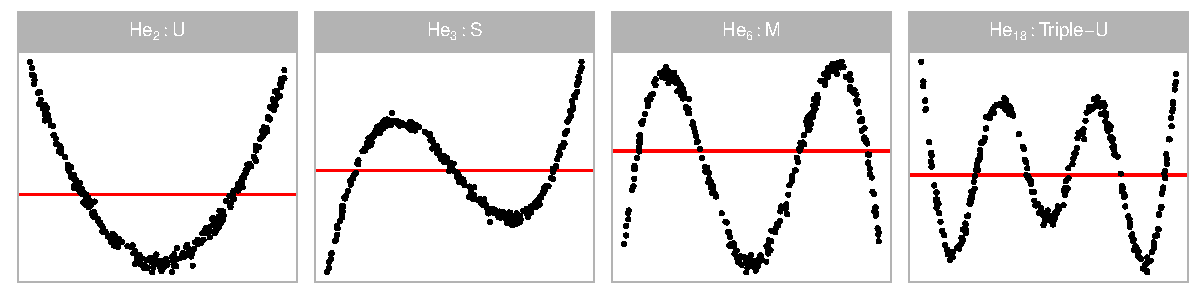
\includegraphics{paper_comparison_files/figure-latex/different-shape-of-herimite-1.pdf}

The range of \(\sigma\) was chosen so that estimates of the power would
produce reasonably continuous power curves, comparable to that
calculated for the conventional test. The values for
\(\boldsymbol{X}_{raw}\) were generated randomly and independently from
one of the following four distributions: (1) \(U(a = -1, b = 1)\), (2)
\(N(\mu = 0, \sigma = 0.3)\), (3) \(lognormal(\mu = 0, \sigma = 0.6)/3\)
and (4) \(u\{a = 1, b = 5\}\). The uniform and the normal distribution
are symmetric and commonly assumed. The adjusted log-normal distribution
provides skewered density. The discrete uniform distribution provides
discreteness in residual plot, which could enrich the pool of visual
patterns. Three replications are made for each of the parameter values
shown in {[}table ref here{]} and thus, 192 different lineups. For each
lineup, the null model was fit to the actual dataset to obtain residuals
and parameter estimates. The actual data plot was drawn as standard
residual plot with raw residuals on the y-axis and fitted values on the
x-axis. The 19 null datasets were generated by the residual rotation
technique, and plotted in the same way. The actual data plot was
randomly placed among these null dadta plots to produce the lineup.
{[}figure ref here{]} is an example of one of these lineups. It was
generated for \(n = 1\), \(\sigma = 1\), \(j = 1\), \(X_{raw} \sim N\).
For this lineup, x out of k observers picked the actual data plot. Each
lineup is evaluated by 5 different subjects to provide reasonable
estimates of the p-value.

To satisfy the plan described above, we needed to recruit at least 160
subjects.

\hypertarget{results}{%
\section{Results}\label{results}}

\hypertarget{data-cleaning}{%
\subsection{Data cleaning}\label{data-cleaning}}

Participants recruited from Prolific are paid for their efforts. Some
participants will try to maximize their earnings for minimum effort,
which can affect the result from the data. For the purpose of
identifying these participants and cleaning the data, two attention
checks are included in the block of 20 lineups. If the subject failed to
identify at least one of the actual data plot in those attention checks,
we reject the submission and the subject will not be paid. All attention
checks are removed from the final data. {[}table ref here{]} tabulates
the number of subjects, genders, and lineups evaluated after applying
the data screening procedure.

\hypertarget{model-fitting}{%
\subsection{Model fitting}\label{model-fitting}}

For each parameter combination, effect \(E\) is derived as
\(E = \frac{1}{2}(\boldsymbol{R}_a\boldsymbol{X}_b)'diag(\sigma^2\boldsymbol{R}_a)\boldsymbol{R}_a\boldsymbol{X}_b\)
from the Kullback-Leibler divergence. {[}KL divergence ref here{]} (The
derivation is provided in {[}appendix ref here{]}.). The logistic
regression is fit using \(E\) as the only fixed effect covariate

\hypertarget{demographic-summary}{%
\section{Demographic summary}\label{demographic-summary}}

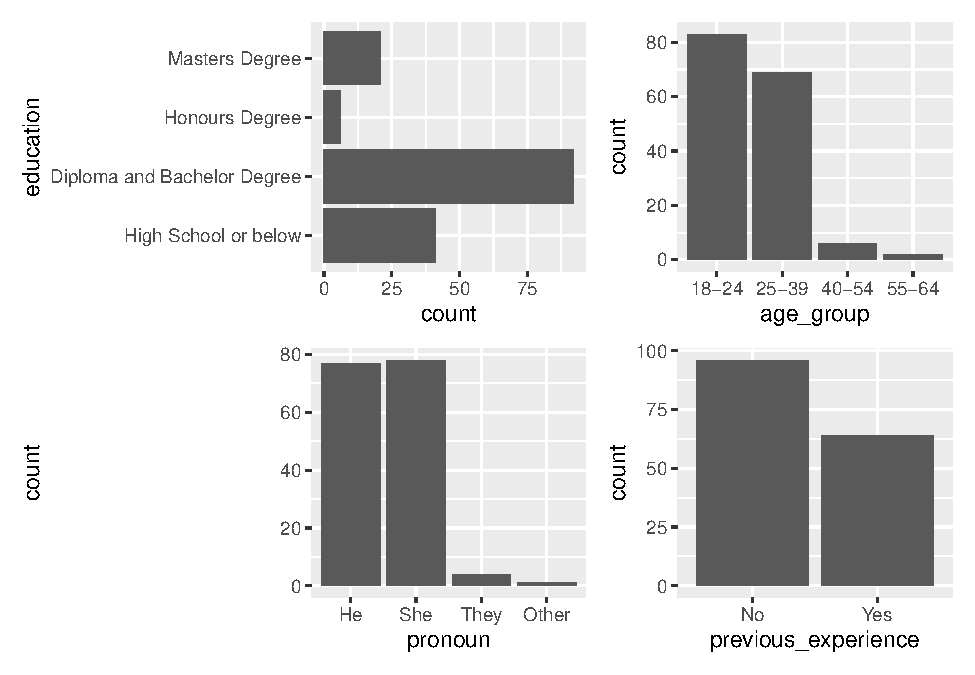
\includegraphics{paper_comparison_files/figure-latex/unnamed-chunk-2-1.pdf}

\hypertarget{data-processing}{%
\section{Data processing}\label{data-processing}}

\hypertarget{results-1}{%
\section{Results}\label{results-1}}

\hypertarget{overview-of-the-data}{%
\subsection{Overview of the Data}\label{overview-of-the-data}}

We collected 400 lineup evaluations made by 20 participants in
experiment I and 880 lineup evaluations made by 44 participants in
experiment II. In total, 442 unique lineups were evaluated by 64
subjects. In experiment I, one of the participants skipped all 20
lineups. Hence, the submission was rejected and removed from the
dataset. In experiment II, there was a participant failed one of the two
attention checks, but there was no further evidence of low-effort
throughout the experiment. Therefore, the submission was kept.

\hypertarget{power-comparision}{%
\subsection{Power comparision}\label{power-comparision}}

\begin{enumerate}
\def\labelenumi{\arabic{enumi}.}
\tightlist
\item
  power (visual test vs.~conventional test) (visual test most different
  one (everything test, any departure)) plot figure in a paper, desc,
  exp
\item
  investigate the difference (gap), give examples
\item
  conventional is too sensitive
\item
  make conventional less sensitive (vary alpha)
\end{enumerate}

To model the power of visual test, 10 logistic regression were fit for
different number of evaluations ranged from one to five and two
different types of simulation setting. All 10 models used natural
logarithm of the effect size as the only fixed effect, and whether the
test successfully rejects the null hypothesis as the response variable.
Given the way we define the effect size, it was expected that with
larger effect size, both conventional test and visual test will have
higher probability in rejecting the null hypothesis when it is not true.
The modelling result summarized in \ref{tab:powerglmcubic} and
\ref{tab:powerglmheter} aligned with the expectation as the coefficients
of natural logarithm of the effect size are positive and significant
across all 10 models.

Figure \ref{fig:power-com} illustrates the fitted models, while
providing the local constant estimate of the power of F-test and
Breusch--Pagan test for comparison. Data for the conventional test is
simulated under the model setting described in section \ldots{} and
5000000 samples are drawn for both cubic and heteroskedasticity model.
From Figure \ref{fig:power-com}, it can be observed that the fitted
power of visual test increased as the number of evaluations increased
for both cubic and heteroskedasticity model.

For heteroskedasticity model, this phenomenon was more obvious as the
power of visual tests with evaluations greater than two were always
greater than those with evaluations smaller than two.

For cubic model, the separation between curves was small. The estimated
power of visual tests with three to five evaluations were almost
identical to each other in regards of effect size. In addition, all five
curves peaked at one as effect size increased, suggesting that
identification of non-linearity as a visual task can be completed
reliably by human as long as the departure from null hypothesis is large
enough.

As shown in Figure \ref{fig:power-com}, both F-test and Breusch--Pagan
test generally possessed greater power than visual test. A visual tests
is a collection of test against any alternatives that would create
visual discoverable features, while a conventional test is usually
targeting at a pre-specified alternative. Considering the data
generating process of the model defect was known and controlled in this
research, where all other alternatives have been eliminated except the
one we concerned, the result was suggested that conventional tests were
more sensitive to violations of linearity and homoscedasticity
assumption than visual tests.

It was also found that there was a noticeable gap between curves of the
conventional test and the visual test at around
\(log(\text{effect size}) = 0\) for the cubic model and
\(log(\text{effect size}) = 2.5\) for the heteroskedasticity model,
where the differences in power were greater than 0.6. We further
analysed the lineups with correspoding effect sizes. Figure
\ref{fig:cubic-hard} and \ref{fig:heter-hard} showed that human was
indeed hard to identify the patterns at this level of difficulty. The
visual difference between the true data plot and null plots were almost
unnoticeable.

\hypertarget{effect-of-parameters-on-power-of-the-visual-test}{%
\subsection{Effect of parameters on power of the visual
test}\label{effect-of-parameters-on-power-of-the-visual-test}}

The previous section focuses on the change of effect size relative to
the power of the visual test. However, effect size is only a one
dimensional summarisation of parameters used in data simulation.
Individual factor embedded in the simulation process should also be
analysed.

In cubic model, two major factors that influencing the strength of the
signal are \(a\) and \(b\). Figure \ref{fig:power-com-cubic-a} and
\ref{fig:power-com-cubic-a} illustrates 30 different logistic
regressions fit for different number of evaluations and different number
of observations \(n\). The regressor used in these models was
\(|a|/\sigma\) since the noise level \(\sigma\) needed to be taken into
account. From the figures, we can observe \ldots{}

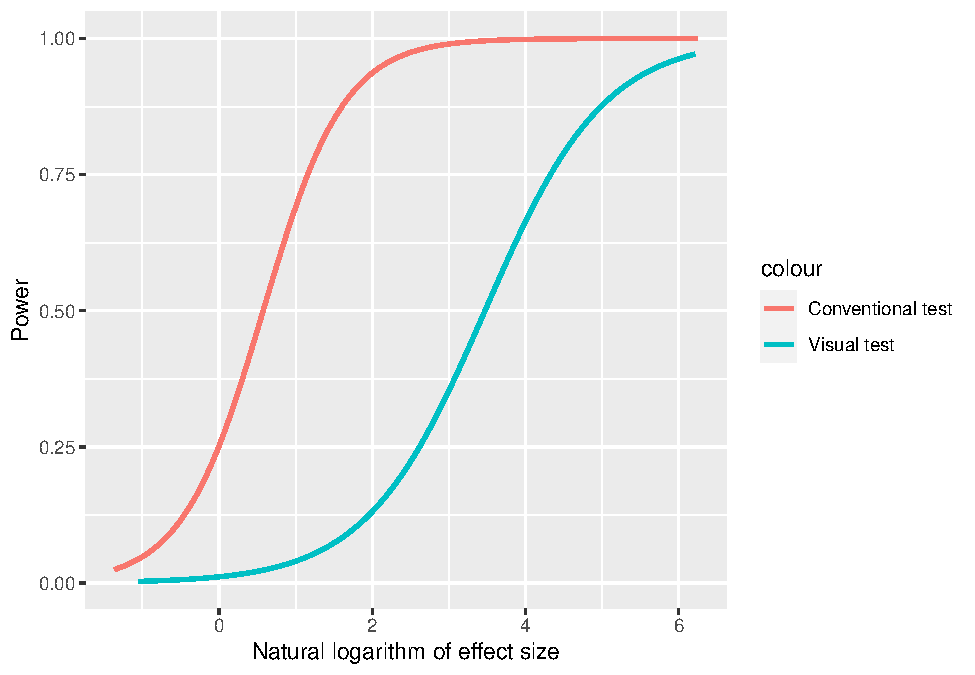
\includegraphics{paper_comparison_files/figure-latex/power-vs-log-effect-size-1.pdf}

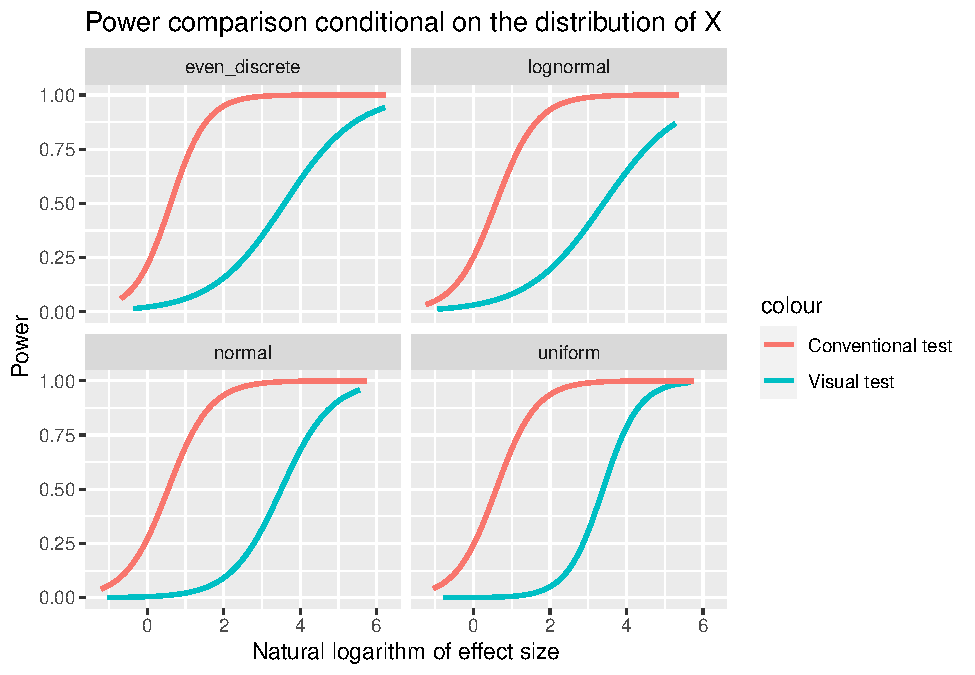
\includegraphics{paper_comparison_files/figure-latex/power-vs-log-effect-size-given-x-dist-1.pdf}

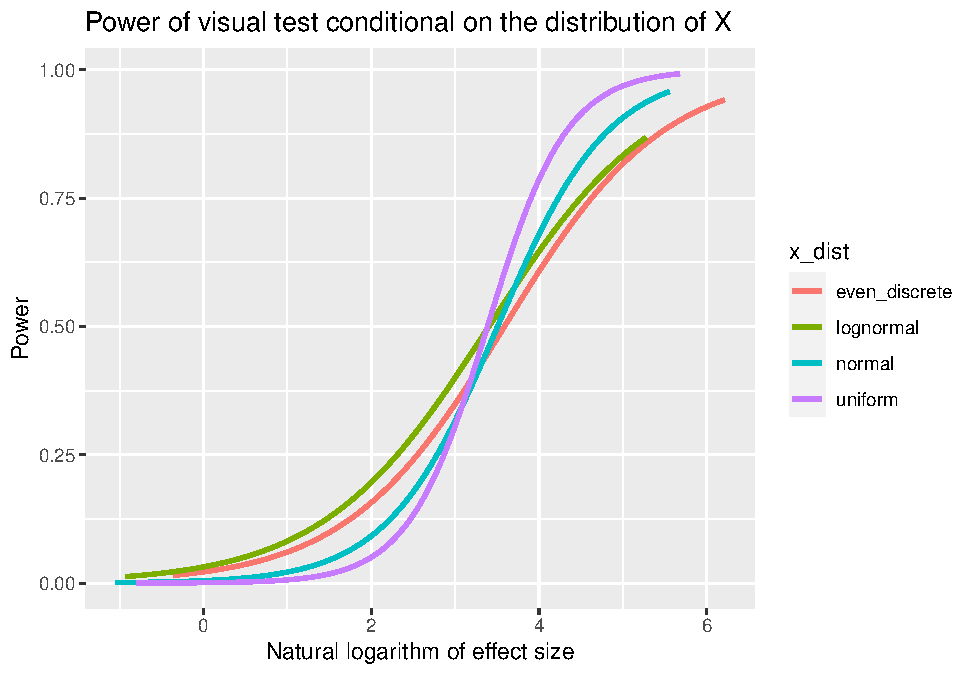
\includegraphics{paper_comparison_files/figure-latex/power-of-visual-test-given-x-dist-1.pdf}

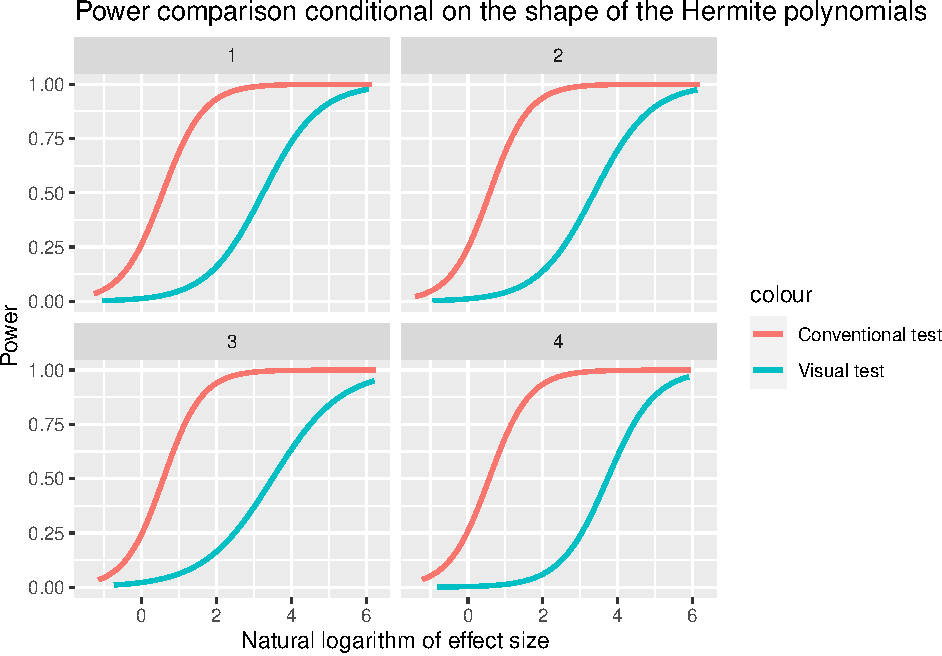
\includegraphics{paper_comparison_files/figure-latex/power-vs-log-effect-size-given-shape-1.pdf}

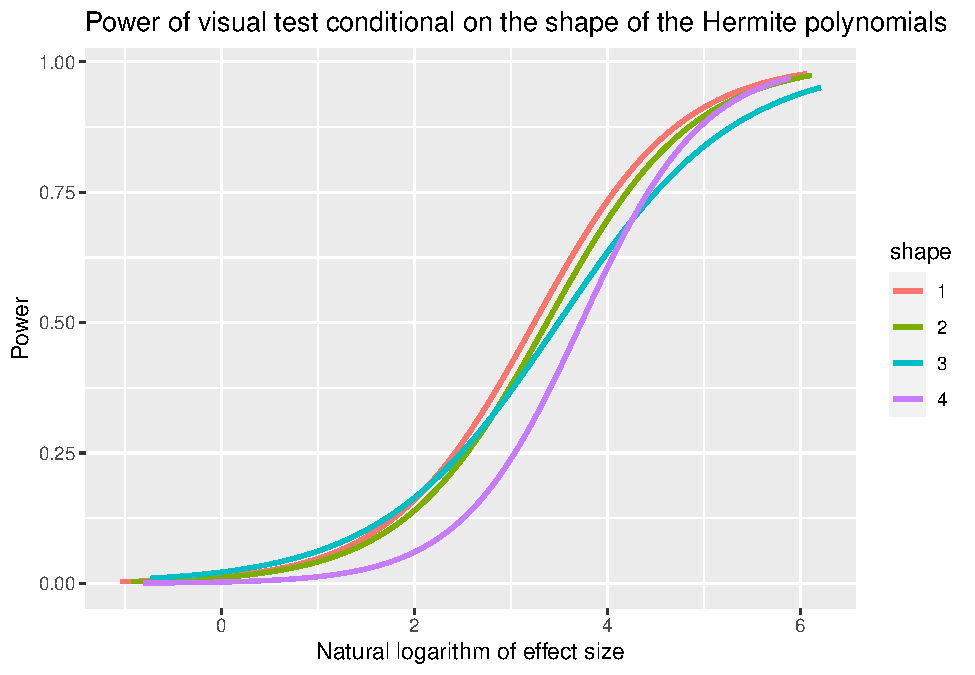
\includegraphics{paper_comparison_files/figure-latex/power-of-visual-test-given-shape-1.pdf}

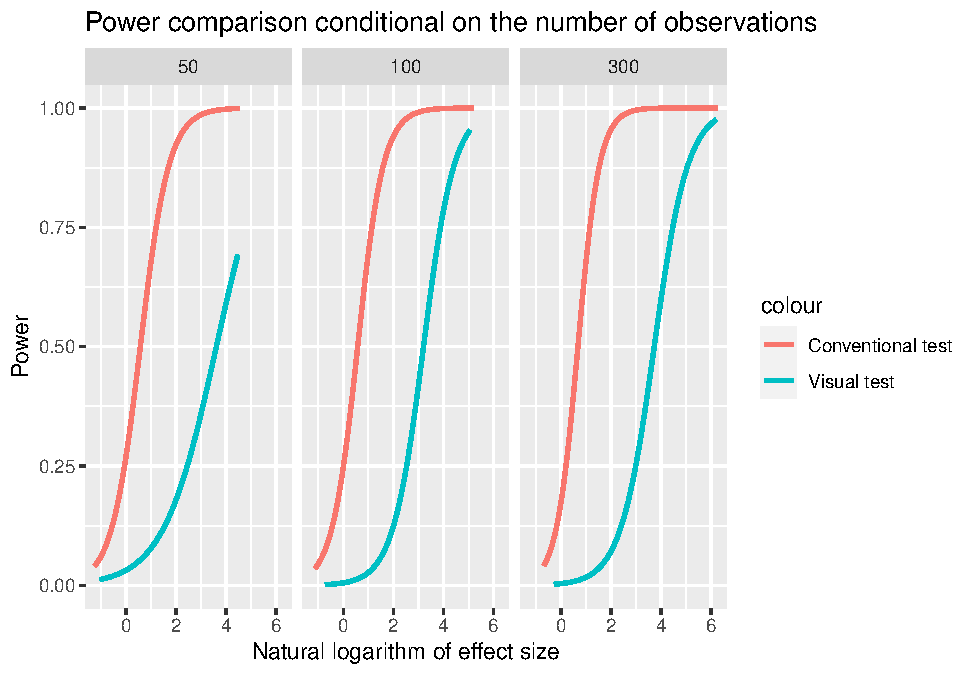
\includegraphics{paper_comparison_files/figure-latex/power-vs-log-effect-size-given-number-of-observations-1.pdf}

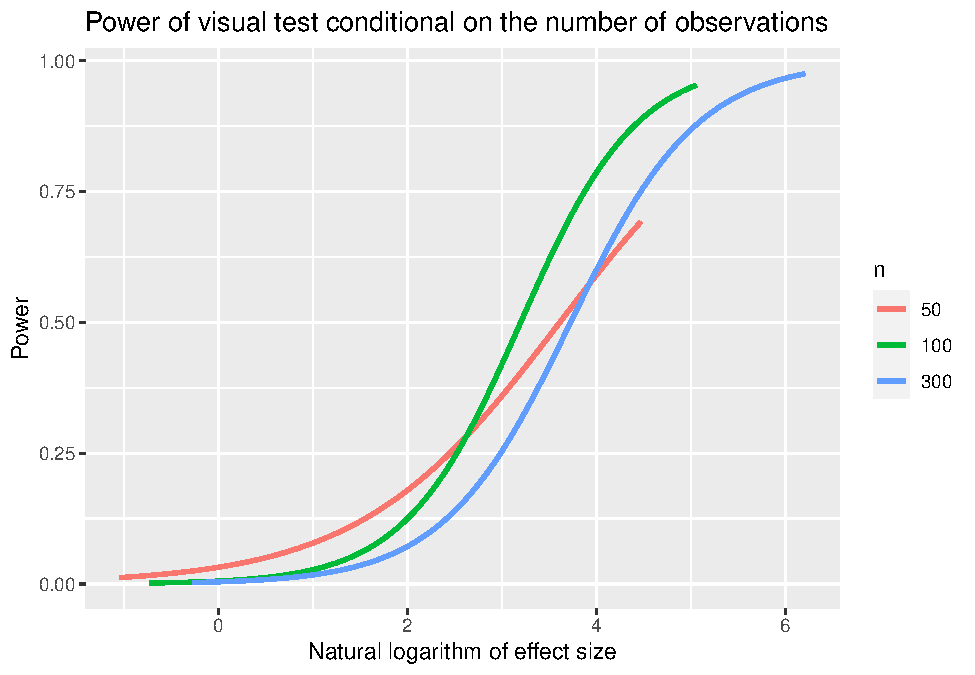
\includegraphics{paper_comparison_files/figure-latex/power-of-visual-test-given-number-of-observations-1.pdf}

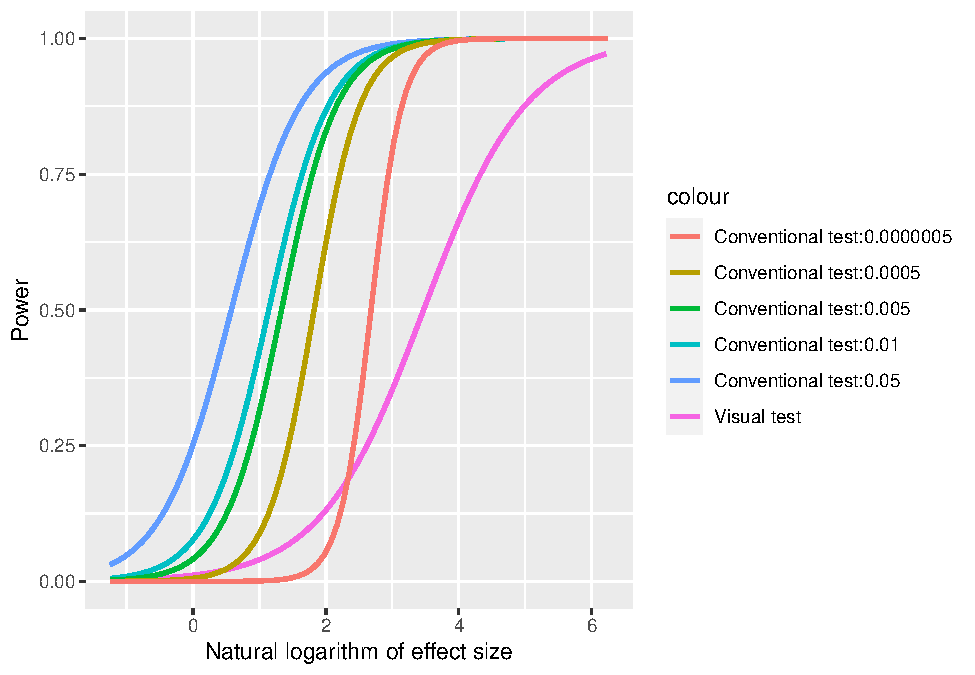
\includegraphics{paper_comparison_files/figure-latex/unnamed-chunk-3-1.pdf}

\bibliographystyle{tfcad}
\bibliography{paper.bib}




\end{document}
